As we saw, protein folding is actually a hard task.
The application of PERM algorithm gave better results by incrementing the number of iteration, but required a lot of computational time, e.g. 5 hours for $10^8$ iterations of Fig. \ref{fig:18_2}.
Furthermore, the application of the \emph{CPSP-tools} library managed to compute the energies in the 3D case, where the other algorithm failed.
However, this approach is not sustainable because the result's uncertainty will grow up as the protein length increases and even well-optimized brute force algorithm will suffer the curse of dimensionality.

In sec \ref{sec:RL} we explained how simple Reinforcement Learning  constitutes a \emph{smart} (AI-wise) version of the PERM algorithm, but it still falls short from a computational point of view.
By comparing performances it emerged that the best models for predicting protein structure in the HP approximation are Deep Q-Networks, which are a particular kind of Reinforcement Learning algorithms that exploit neural networks.
It is important to underline that despite this kind of models have already outperformed classical algorithms their research field is still thriving and there still is room for improvement.
Therefore, a solution to the HP model should be searched into the Artificial Intelligence field.
Solutions based on deep reinforcement learning, and in general in the A.I. field, are more sustainable and give better results.

On the other hand, a solution to the general protein folding problem is given by bioinformatics.
Bioinformatics is conceptualizing biology in terms of molecules and applying ``informatics techniques'' to understand and organize the information associated with these molecules, on a large scale \cite{bioinfo}.
The aims of bioinformatics are multiple.
Firstly, well-organized data allow researches to access existing information and to submit new entries as they are produced.
Secondly, it develops tool and resources useful for the analysis of these data.
The development of these tools requires a lot of knowledge in biology, informatic and also physics and mathematics.
\begin{figure}[H]
    \centering
    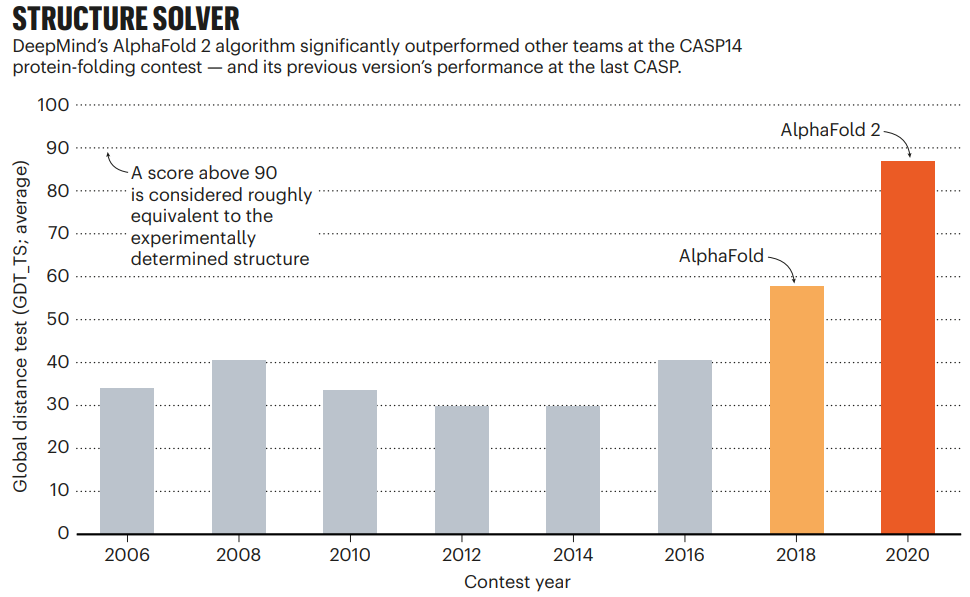
\includegraphics[width=.6\textwidth]{./img/alphafold.png}
    \caption{\emph{Protein folding algorithms' accuracy through time \cite{alphafold}.}}
    \label{fig:alphafold}
\end{figure}
Two example of intelligences that are giving many good results are AlphaFold and AlphaFold2 by Google.
In particular, the second one reached a precision level comparable to the experimental one, as wee can see from Fig \ref{fig:alphafold}.
The future of this topic seems to be linked to research whose goal is to expand the protein databases underlying these intelligences.
